\chapter{过渡金属与配合物}\label{ch:b2:coordination-complexes}

1893 年，年仅二十六岁的化学家阿尔弗雷德·维尔纳着手解释一个谜题。
氯化钴(III)与氨形成四种化合物，即 \ce{CoCl3.6NH3}、
\ce{CoCl3.5NH3} 以及两种化学式为 \ce{CoCl3.4NH3} 的化合物，其中一种为绿色，一种为紫色。
硝酸银立即沉淀出第一种化合物的全部三个氯离子，第二种沉淀出两个，
最后两种各只沉淀出一个。维尔纳的解释——六个基团
以八面体顶点的方式围绕金属，其余基团位于外界
——开创了配位化学。本章把本科一年级分册中的配合物
扩展到其几何构型、异构体、命名，以及可预测哪些金属羰基化合物存在的
电子计数方法。

\begin{recall}
本科一年级分册回顾：配合物、中心原子、配体、多齿配体、螯合物、
形成常数、配位数；过渡金属离子的电子排布，
即先失去 $n$s 电子；路易斯酸碱、
配位键；价层电子对互斥模型；氧化数；对映异构体。\Cref{ch:b2:atomic-orbitals}：
d 轨道，以及 4s 与 3d 能级的顺序。
\end{recall}

\begin{omfigure}
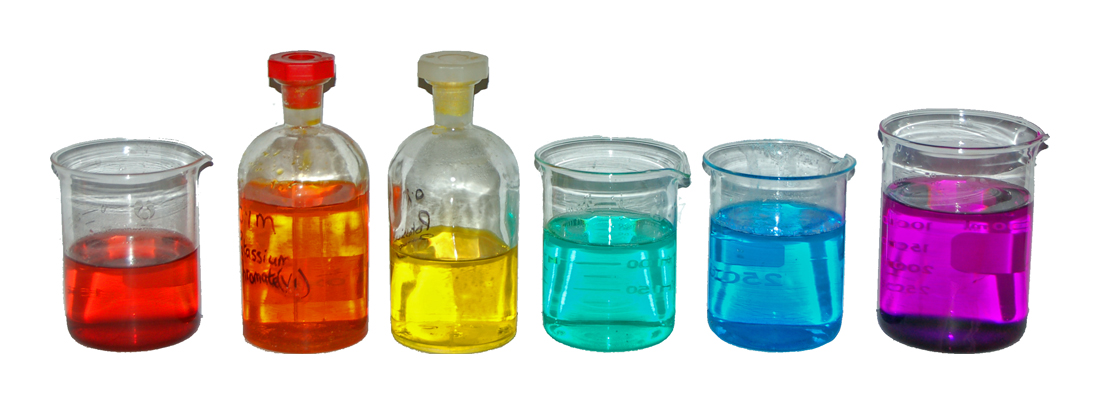
\includegraphics[width=0.8\linewidth]{images/book3/tm-solutions.jpg}

{\small 过渡金属化合物的水溶液，从左至右依次为
硝酸钴(II)、重铬酸钾、铬酸钾、氯化镍(II)、
硫酸铜(II)和高锰酸钾。钴、镍
和铜溶液的颜色来自其水合配合物。（照片：Benjah-bmm27，
公有领域，维基共享资源。）}
\end{omfigure}

\section{d 区}

\begin{definition}[过渡元素]\label{def:b2:coordination-complexes:transition-element}
若某元素的原子或其某一常见离子的
d 亚层部分填充，则称该元素为\emph{过渡元素}\index{过渡元素}。元素的此类离子若在其
d 轨道上有 $n$ 个电子，则具有\emph{$d^n$ 组态}\index{$d^n$ 组态}。
\end{definition}

\begin{proposition}[d 电子计数]\label{prop:b2:coordination-complexes:dn}
设过渡金属离子 $\mathrm M^{m+}$ 位于编号为 $g$（3 至 12）的族，
则其具有 $d^n$ 组态，且 $n = g - m$。
\end{proposition}

\begin{proof}
中性原子在前一稀有气体之外有 $g$ 个电子，分布在 $n$s 与
$(n - 1)$d 轨道上。在离子中，d 轨道的能级低于 s 轨道
（见\cref{ex:b2:atomic-orbitals:iron}），故剩余的 $g - m$ 个价电子
全部为 d 电子。
\end{proof}

例如 \ce{Fe^2+}（第 8 族）为 $d^6$，\ce{Cu^2+}（第 11 族）为 $d^9$，\ce{Co^3+}（第 9 族）
为 $d^6$，\ce{Pt^2+}（第 10 族）为 $d^8$。

\section{配体}

\begin{definition}[齿数]\label{def:b2:coordination-complexes:denticity}
配体的\emph{齿数}\index{齿数}是与同一中心原子相键合的
原子数目。\emph{单齿配体}\index{单齿配体}通过一个原子
配位（如 \ce{H2O}、\ce{NH3}、\ce{Cl-}、\ce{CO}），\emph{双齿配体}\index{双齿配体}
通过两个原子配位（乙烷-1,2-二胺，记作 en；
乙二酸根离子，记作 ox）。\emph{桥联配体}\index{桥联配体}同时与
两个金属原子结合。\emph{两可配体}\index{两可配体}可通过
两种不同原子中的任一种结合，例如亚硝酸根离子（通过 N 或 O）
或硫氰酸根离子（通过 S 或 N）。
\end{definition}

\begin{definition}[配位层]\label{def:b2:coordination-complexes:coordination-sphere}
配合物的\emph{配位层}\index{配位层}是由
中心原子及与之键合的配体组成的集合，写在方括号内；方括号外的离子
为抗衡离子，不与金属原子键合。
\end{definition}

\begin{omfigure}
\setchemfig{atom sep=2.2em}
\chemfig{M*5(-H_2N-CH_2-CH_2-NH_2-)}
\qquad
\chemfig{M*5(-O-(=O)-(=O)-O-)}
\qquad
\chemfig{N(-[:120]CH_2COO^{-})(-[:240]CH_2COO^{-})-CH_2-CH_2-N(-[:60]CH_2COO^{-})(-[:-60]CH_2COO^{-})}

\medskip
{\small 螯合配体。左：乙烷-1,2-二胺（en），双齿，通过其两个
氮原子配位。中：乙二酸根离子（ox），双齿，通过两个氧原子配位。右：
EDTA 阴离子，它以两个氮原子和四个
羧酸根氧原子包裹金属离子（六齿配体）。}
\end{omfigure}

\section{配位数与几何构型}

配位数最常见的是二、四和六。银(I)与金(I)形成
直线型配合物（\ce{[Ag(NH3)2]+}）；四个配体形成四面体
（\ce{[CoCl4]^2-}、\ce{[Zn(NH3)4]^2+}）或正方形（\ce{[PtCl4]^2-}、\ce{[Ni(CN)4]^2-}）；
五配位形成三角双锥（\ce{Fe(CO)5}）；六配位最为常见，形成
八面体。

\begin{omfigure}
\begin{tikzpicture}[font=\small]
  \node[omligand] at (-0.8,0) {}; \node[omligand] at (0.8,0) {};
  \draw[thick, black!70] (-0.8,0) -- (0.8,0); \node[ommetal] at (0,0) {};
  \node at (0,-1.5) {直线形，2};
  \pic at (3,0) {omtetrahedron}; \node at (3,-1.5) {四面体形，4};
  \pic at (6,0) {omsquareplanar}; \node at (6,-1.5) {平面正方形，4};
  \pic at (9,0) {omtbp}; \node[align=center] at (9,-1.65) {三角 \\双锥，5};
  \pic at (12,0) {omoctahedron}; \node at (12,-1.5) {八面体形，6};
\end{tikzpicture}

{\small 常见配位几何构型（金属为橙色，配体为灰色；虚线
键指向纸面背后）。}
\end{omfigure}

价层电子对互斥模型使中心原子的电子对尽可能彼此远离，
在此失效：$d^8$ 离子（如 \ce{Pt^2+}）带有四对 d 电子，并有四个
配体相连，但其配合物为平面正方形，而非四面体形或八面体形。
d 电子并非推开配体的定域电子对：其能量
取决于几何构型，这一依赖关系将在下一章计算。

\begin{proposition}[平面正方形 $d^8$]\label{prop:b2:coordination-complexes:square-planar}
第二、第三过渡系中 $d^8$ 离子的四配位配合物
（\ce{Pd^2+}、\ce{Pt^2+}、\ce{Au^3+}）均为平面正方形。
\end{proposition}

\admitted

其解释即配体引起的 d 能级分裂，
在\cref{ch:b2:ligand-field}中给出。

\section{同分异构体}

\begin{definition}[配合物的同分异构体]\label{def:b2:coordination-complexes:isomers}
在八面体配合物 $\mathrm{MA_3B_3}$ 中，\emph{面式异构体}\index{面式异构体}
的三个 B 配体位于八面体的同一面上，\emph{经式
异构体}\index{经式异构体}位于经线位置（三个位置处于过
金属的同一平面内）。\emph{键合异构体}\index{键合异构体}的区别在于\omterm{def:b2:coordination-complexes:denticity}{两可配体}通过
哪一原子与金属结合。\emph{电离异构体}\index{电离异构体}
与抗衡离子交换一个配体，在溶液中给出不同的离子。
\end{definition}

\begin{proposition}[八面体异构体的计数]\label{prop:b2:coordination-complexes:isomer-count}
在八面体中，$\mathrm{MA_4B_2}$ 有两种异构体（顺式和反式），$\mathrm{MA_3B_3}$ 有
两种（面式和经式），$\mathrm M(\mathrm{AA})_3$ 含三个\omterm{def:b2:coordination-complexes:denticity}{双齿配体}时有
两种对映异构体，即 $\Delta$ 和 $\Lambda$。
\end{proposition}

\begin{proof}
八面体中任意两个位置或相邻（顺式，$90^\circ$），
或相对（反式，$180^\circ$）：对两个 B 配体有两种排布。对三个 B 配体，
或两两皆不互为反式（占据一个面：面式），或恰有一对互为反式（第三个
与这两者均为顺式：经式）；三个两两互为反式的位置并不存在。
对 $\mathrm M(\mathrm{AA})_3$，每个螯合物占据两个顺式位置；三个螯合物
绕三重轴如螺旋桨叶片般旋转，沿该轴观察时顺时针
或逆时针旋转，两者互为镜像，不能重合，
因为该配合物不存在镜面。
\end{proof}

\begin{omfigure}
\begin{tikzpicture}[font=\scriptsize]
  \pic (a) at (0,0) {omoctahedron};
  \node[omligand, fill=omDef!70] at (a-L1) {}; \node[omligand, fill=omDef!70] at (a-L3) {};
  \node at (0,-1.5) {\small 顺式-$\mathrm{MA_4B_2}$};
  \pic (b) at (3,0) {omoctahedron};
  \node[omligand, fill=omDef!70] at (b-L1) {}; \node[omligand, fill=omDef!70] at (b-L2) {};
  \node at (3,-1.5) {\small 反式-$\mathrm{MA_4B_2}$};
  \pic (c) at (6.5,0) {omoctahedron};
  \node[omligand, fill=omThm!70] at (c-L1) {}; \node[omligand, fill=omThm!70] at (c-L3) {}; \node[omligand, fill=omThm!70] at (c-L5) {};
  \node at (6.5,-1.5) {\small 面式-$\mathrm{MA_3B_3}$};
  \pic (d) at (9.5,0) {omoctahedron};
  \node[omligand, fill=omThm!70] at (d-L1) {}; \node[omligand, fill=omThm!70] at (d-L2) {}; \node[omligand, fill=omThm!70] at (d-L3) {};
  \node at (9.5,-1.5) {\small 经式-$\mathrm{MA_3B_3}$};
\end{tikzpicture}

\medskip
\begin{tikzpicture}[font=\scriptsize]
  \foreach \xs/\s/\lab in {0/1/{$\Delta$}, 4.5/-1/{$\Lambda$}} {
    \begin{scope}[xshift=\xs cm, xscale=\s]
      \draw[black!30] (0,0) circle (1.2);
      \foreach \a in {90, 210, 330} {
        \coordinate (p) at (\a:1.1); \coordinate (q) at (\a+70:0.55);
        \draw[very thick, omDef] (\a:1.1) .. controls (\a+30:1.25) and (\a+60:0.9) .. (\a+75:0.55);
        \node[omligand] at (\a:1.1) {}; \node[omligand] at (\a+75:0.55) {};
      }
      \node[ommetal] at (0,0) {};
    \end{scope}
    \node at (\xs,-1.6) {\small \lab};
  }
  \draw[densely dashed] (2.25,-1.3) -- (2.25,1.3);
  \node[anchor=south] at (2.25,1.3) {镜面};
\end{tikzpicture}

{\small 上：$\mathrm{MA_4B_2}$ 的顺式和反式异构体（B 配体为蓝色），面式和\omterm{def:b2:coordination-complexes:isomers}{经式
异构体} $\mathrm{MA_3B_3}$（B 配体为红色）。下：三螯合配合物的两种对映异构体（例如
\ce{[Co(en)3]^3+}），沿三重轴观察，为示意图：每个螯合物（蓝色
弧）连接上、下两个位置，三者朝一个方向（$\Delta$）或另一个方向（
$\Lambda$）旋转。}
\end{omfigure}

\section{命名与电子计数}

\begin{method}[配合物的命名]\label{met:b2:coordination-complexes:naming}
\begin{enumerate}
  \item 在化学式中，以方括号写出\omterm{def:b2:coordination-complexes:coordination-sphere}{配位层}，金属
        居先，配体随后；配合物的电荷标在方括号外。
  \item 命名时，先列配体（阴离子配体在前），并加上倍数词头
        （二、三、四；复杂配体用双、三）：阴离子配体称为
        氯、氰、氧、羟，中性配体称为
        水、氨、羰基。
  \item 然后写金属名，若配合物为阴离子，则称“某酸”（铁酸、
        铜酸、钴酸），并以罗马数字标出其氧化数。
  \item 阳离子命名在阴离子之前：\ce{[Co(NH3)6]Cl3} 命名为
        六氨合钴（III）氯化物，\ce{K4[Fe(CN)6]} 命名为
        六氰合铁（II）酸钾。
\end{enumerate}
\end{method}

\begin{definition}[电子计数]\label{def:b2:coordination-complexes:electron-count}
配合物的\emph{价电子计数}\index{价电子计数}是
金属离子的 d 电子数，加上配体所提供的电子（每个给电子对
提供两个电子）。\emph{18 电子规则}\index{18 电子规则}指出
低氧化态金属与强成键的 $\pi$ 受体
配体（如 \ce{CO}）形成的稳定配合物倾向于具有 18 个价电子。
\end{definition}

\begin{definition}[哈普托数]\label{def:b2:coordination-complexes:hapticity}
配体的\emph{哈普托数}\index{哈普托数}是与金属通过一个连续的
$\pi$ 体系键合的原子数，记作 $\eta^n$：以其 $\pi$ 键键合的乙烯为
$\eta^2$，以全部五个碳原子键合的环戊二烯基为 $\eta^5$。
\end{definition}

\begin{method}[电子计数]\label{met:b2:coordination-complexes:electron-count}
\begin{enumerate}
  \item 将配体按闭壳层物种指定电荷（\ce{Cl-}、\ce{H-}、
        \ce{C5H5-}；\ce{CO}、\ce{PR3}、\ce{NH3} 为中性），并推出金属的
        氧化数。
  \item 数出金属的 d 电子数，$n = g - m$。
  \item 每个给电子对加两个电子：每个\omterm{def:b2:coordination-complexes:denticity}{单齿配体}计一对，
        $\eta^5$-\ce{C5H5-} 加六个，$\eta^6$-苯加六个，$\eta^2$-烯烃加两个。
  \item 金属–金属键中，每个金属各计一个电子。
\end{enumerate}
\end{method}

\begin{proposition}[金属羰基化合物]\label{prop:b2:coordination-complexes:eighteen}
第一过渡系列的稳定二元羰基化合物 \ce{Cr(CO)6}、
\ce{Fe(CO)5}、\ce{Ni(CO)4} 和 \ce{Mn2(CO)10} 均
每个金属原子具有 18 个价电子。
\end{proposition}

\begin{proof}
铬（0），$d^6$，配六个 CO：$6 + 12 = 18$。铁（0），$d^8$，配五个 CO：$8 + 10 = 18$。
镍（0），$d^{10}$，配四个 CO：$10 + 8 = 18$。锰（0），$d^7$，配五个 CO 和一个
Mn--Mn 键：$7 + 10 + 1 = 18$；单体 \ce{Mn(CO)5}（价电子数为 17）不能作为
稳定化合物存在，而会发生二聚化。18 为何更受青睐——金属的九个价轨道
（成键与\omterm{def:b2:diatomic-mos:bonding}{非键轨道}）全部填满——其原因见
\cref{ch:b2:ligand-field}。
\end{proof}

二茂铁 \ce{Fe(\eta^5-C5H5)2}，其中铁（II）离子（$d^6$）位于两个
环戊二烯基阴离子之间，每个提供六个电子：$6 + 12 = 18$。该规则不适用于
多数高氧化态配合物及许多含弱配体的配合物：\ce{[Ti(H2O)6]^3+}
有 13 个电子，\ce{[Cu(H2O)6]^2+} 有 21 个。

\begin{history}[维尔纳与八面体]
\begin{minipage}[t]{0.22\linewidth}
\vspace{0pt}
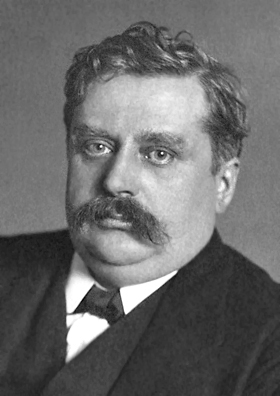
\includegraphics[width=\linewidth]{images/book3/werner.jpg}
\end{minipage}\hfill
\begin{minipage}[t]{0.74\linewidth}
\vspace{0pt}
1893 年，阿尔弗雷德·维尔纳提出，金属除化合价外，还有一个
配位数（即直接围绕其周围的基团数），并认为钴（III）
六个基团位于八面体的顶点。他随后预言了每种
化学式应有的异构体数目，并花了二十年时间制备它们；1911 年，他将一种钴配合物
拆分为两种对映异构体，证明手性并不必依赖
碳原子。他于 1913 年获诺贝尔化学奖。（肖像出自诺贝尔奖年鉴，
1914 年，公有领域，维基共享资源。）
\end{minipage}
\end{history}

\section{练习}

\begin{exercise}[$\star$]\label{exo:b2:coordination-complexes:1}
求 \ce{Ti^3+}、\ce{V^3+}、\ce{Cr^3+}、\ce{Mn^2+}、\ce{Fe^3+}、
\ce{Co^2+}、\ce{Ni^2+} 和 \ce{Zn^2+} 的 $d^n$ 组态。
\end{exercise}

\begin{exercise}[$\star$]\label{exo:b2:coordination-complexes:2}
求下列配体的\omterm{def:b2:coordination-complexes:denticity}{齿数}：水、乙烷-1,2-二胺、乙二酸根离子、EDTA 和
硫氰酸根离子，并指出哪一个为\omterm{def:b2:coordination-complexes:denticity}{两可配体}。
\end{exercise}

\begin{exercise}[$\star$]\label{exo:b2:coordination-complexes:3}
命名 \ce{[Cu(NH3)4]SO4}、\ce{K3[Fe(CN)6]}、\ce{[CoCl2(NH3)4]Cl} 和
\ce{[Ni(CO)4]}。
\end{exercise}

\begin{exercise}[$\star$]\label{exo:b2:coordination-complexes:4}
预测 \ce{[Ag(NH3)2]+}、\ce{[CoCl4]^2-}、\ce{[PtCl4]^2-} 和
\ce{[Fe(H2O)6]^2+} 的几何构型。
\end{exercise}

\begin{exercise}[$\star\star$]\label{exo:b2:coordination-complexes:5}
平面正方形的 \ce{[PtCl2(NH3)2]} 有多少种异构体？画出它们。（其中一种
为顺铂，是一种抗癌药物。）
\end{exercise}

\begin{exercise}[$\star\star$]\label{exo:b2:coordination-complexes:6}
计算 \ce{Cr(CO)6}、\ce{Fe(CO)5}、\ce{Ni(CO)4}、
\ce{V(CO)6} 和 \ce{Mn2(CO)10} 的价电子数，哪一个违反该规则，它又如何表现？
\end{exercise}

\begin{exercise}[$\star\star$]\label{exo:b2:coordination-complexes:7}
计算二茂铁与二茂钴 \ce{Co(C5H5)2} 的价电子数。哪一个
更易被氧化，并氧化成什么？
\end{exercise}

\begin{exercise}[$\star\star$]\label{exo:b2:coordination-complexes:8}
EDTA 形成的镍（II）配合物的 $\log_{10}K = 20.5$，远高于
镍与六个各自独立的氮或氧给电子原子配位所形成的配合物。请解释
这一螯合效应，从螯合剂取代六个水分子时释放出的
粒子数的角度加以说明。
% ledger: logb:Ni-edta
\end{exercise}

\begin{exercise}[$\star\star$]\label{exo:b2:coordination-complexes:9}
画出 \ce{[Co(NO2)(NH3)5]^2+} 的两种\omterm{def:b2:coordination-complexes:isomers}{键合异构体}。
\end{exercise}

\begin{exercise}[$\star\star\star$]\label{exo:b2:coordination-complexes:10}
\ce{[CoCl2(en)2]+} 有多少种立体异构体？其中哪些是手性的？
\end{exercise}

\begin{exercise}[$\star\star\star$]\label{exo:b2:coordination-complexes:11}
对于 $\mathrm{MA_4B_2}$，计算按平面六边形及
三角棱柱排布六个配体时预测的异构体数目，并说明实际找到的异构体数如何
在两种几何构型之间作出判断。
\end{exercise}

\begin{exercise}[$\star\star\star$]\label{exo:b2:coordination-complexes:12}
数出 \ce{[RhCl(PPh3)3]} 和 \ce{[IrH(CO)(PPh3)3]} 的价电子数
（\ce{PPh3} 为二电子给体，\ce{H-} 作为氢负离子）。哪一个还能再结合两个
配体？
\end{exercise}

\section{问题：维尔纳的钴氨配合物}

\begin{problem}[{周末问题——四种三氯化钴氨合物及其释放的氯离子，
各自的化学式列于括号中，四氨合物的两种异构体及其所证明的几何构型，
以及三螯合物的旋光性}]
\label{pb:b2:coordination-complexes:1}
数据：四种化合物 A \ce{CoCl3.6NH3}（橙黄色），B \ce{CoCl3.5NH3}
（紫色）。C 和 D \ce{CoCl3.4NH3}（绿色和紫色）。加入过量硝酸银后，
1 摩尔 A 沉淀出 3 摩尔 \ce{AgCl}，B 沉淀出 2 摩尔，C 和 D 各沉淀出 1 摩尔。
摩尔电导率表明，每个化学式单元分别产生 4、3、2 和 2 个离子。

\medskip
\noindent\textbf{第一部分——氯离子与离子。}
\begin{enumerate}
  \item 哪些氯化物会立即与银离子反应？
  \item 每种化合物中有多少个氯与钴成键？
  \item 将离子数与电导数据进行核对。
  \item 四种化合物中钴的氧化数各是多少？
  \item 其 $d^n$ 组态是什么？
  \item 每种化合物中钴共结合多少个配体？
\end{enumerate}

\medskip
\noindent\textbf{第二部分——化学式与命名。}
\begin{enumerate}[resume]
  \item 用方括号写出 A、B、C 和 D。
  \item 命名 A 和 B。
  \item 命名 C 和 D 的阳离子。
  \item C 和 D 属于哪一类异构体？
  \item 化合物 \ce{CoCl3.3NH3} 是什么，它会电离出多少个离子？
  \item 该化合物在八面体中可能有多少种异构体？
\end{enumerate}

\medskip
\noindent\textbf{第三部分——几何构型。}
\begin{enumerate}[resume]
  \item 在八面体中画出顺式和反式的 \ce{[CoCl2(NH3)4]+}。
  \item 计算六个配体位于平面六边形顶点时，预测的
        \ce{[CoCl2(NH3)4]+} 异构体数目。
  \item 计算三棱柱构型所预测的异构体数目。
  \item 维尔纳从未发现超过两种异构体。这证明了什么？
  \item 这一证明是否完备？若出现第三种异构体，意味着什么？
  \item 已知顺式异构体可转化为
        与乙二酸根形成的螯合物，而反式异构体不能，试判断 C 和 D 中哪一个是顺式的。
\end{enumerate}

\medskip
\noindent\textbf{第四部分——旋光性。}
\begin{enumerate}[resume]
  \item 画出 \ce{[Co(en)3]^3+}。
  \item 它是否有镜面？是否有对称中心？
  \item 它有多少种立体异构体？
  \item 将这种阳离子拆分为对映异构体，证明了什么？
  \item \ce{[CoCl2(en)2]+} 的顺式形式是否手性？反式形式呢？
  \item 维尔纳拆分一种完全不含碳的配合物，为什么重要？
  \item 写出八面体所预测的 \ce{[CoCl2(NH3)4]+} 异构体数目，
        以及平面六边形和三棱柱所预测的数目。
\end{enumerate}
\end{problem}
